\noindent\textbf{Solution.} The longitudinal displacement is uniform over each cross section, and the bar undergoes small axial strain. For a uniform, linearly elastic bar, the force \(N=A\sigma\) acts on an element of mass \(\rho A\,dx\).

\begin{figure}[H]
\centering
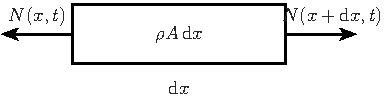
\includegraphics[width=0.55\linewidth]{figures/generated/solutions/C6_fbd.pdf}
\caption{Axial forces on an infinitesimal bar element.}
\end{figure}

Newton's law and the constitutive relation are
\[
N(x+dx,t)-N(x,t)=\rho A\,dx\,u_{tt},\qquad
\sigma=E\epsilon=E u_x.
\]
Dividing by \(dx\), taking its limit, and substituting \(N=EAu_x\) yields
\[
EAu_{xx}=\rho A u_{tt},\qquad
c=\sqrt{\frac E\rho},\qquad u_{tt}=c^2u_{xx}.
\]
This is the slender-bar wave equation in the course notes, Section 1, Eqs. (13)--(16). With \(u=U(x)e^{-i\omega t}\), \(\gamma=\omega/c\), and \(U=e^{sx}\), the spatial equation and characteristic roots are
\[
U''+\frac{\omega^2}{c^2}U=0,\qquad s^2+\gamma^2=0,\qquad s=\pm i\gamma.
\]
Consequently, the complex displacement and its equivalent trigonometric form are
\[
u(x,t)=\left(A_1e^{i\gamma x}+A_2e^{-i\gamma x}\right)e^{-i\omega t}
=\left(C_1\cos\gamma x+C_2\sin\gamma x\right)e^{-i\omega t}.
\]
The term \(A_1e^{i(\gamma x-\omega t)}\) travels toward increasing \(x\), and \(A_2e^{-i(\gamma x+\omega t)}\) travels toward decreasing \(x\). Their phase velocities are \(+c\) and \(-c\), respectively. Physical displacement is the real part.
